\documentclass{article}
\usepackage[colorlinks,bookmarksopen,bookmarksnumbered,citecolor=red,urlcolor=red]{hyperref}
\usepackage[cm]{fullpage}
\usepackage{amsmath,amssymb}
\usepackage{algorithm,algorithmic}
\usepackage{graphicx}
\title{Rare event calculation with path integrals}
\date{\today}
\begin{document}
\maketitle
%%%%%%%%%%%%%%%%%%%%%%%%%%%%%%%%%%%%%%%%%%%%%%%%%%%%%%%%%%%%%%%%%%%%%%%%
\section{Algorithm}
%%%%%%%%%%%%%%%%%%%%%%%%%%%%%%%%%%%%%%%%%%%%%%%%%%%%%%%%%%%%%%%%%%%%%%%%
%%%%%%%%%%%%%%%%%%%%%%%%%%%%%%%%%%%%%%%%%%%%%%%%%%%%%%%%%%%%%%%%%%%%%%%%
\subsection{SDE and path integral formulation of transition probability}
%%%%%%%%%%%%%%%%%%%%%%%%%%%%%%%%%%%%%%%%%%%%%%%%%%%%%%%%%%%%%%%%%%%%%%%%
Consider the SDE
\begin{equation}
dx = -\frac{\partial V}{\partial x}dt+\sigma\;dW
\end{equation}
A finite difference discretisation with stepsize $h$ is for example (forward Euler)
\begin{equation}
x_{n+1} = x_h - hV'(x_n) + \sigma \sqrt{h}\xi_{n+1/2}
\end{equation}
with unit normal random variable $\xi_{n+1/2}\sim\mathcal{N}(0,1)$. Hence the transition probability (density) for going from $x_n$ to $x_{n+1}$ in a timestep of size $h$ is
\begin{equation}
P_h(x_{n+1},x_n) = \frac{1}{\sqrt{2\pi\sigma^2 h}}
\exp\left[
-\frac{\left(x_{n+1}-x_n+hV'(x_n)\right)^2}{2\sigma^2 h}
\right]\label{eqn:transition_probability}.
\end{equation}
The following discussion, however, is independent of the numerical timestepping method, and we only assume that the transition probability (density) in Eq. (\ref{eqn:transition_probability}) is defined.

We want to know the finite time transition probability (density) for a particle starting at $x=a$ at time $t=0$ and ending at $x=b$ at time $t=T>0$ which can be written as the path-integral
\begin{equation}
P(b,a) = \lim_{h\rightarrow 0}
\int\dots\int
P_h(b,x_{n-1})P_h(x_{n-1},x_{n-2})\cdot\dots\cdot
P_h(x_2,x_1)P_h(x_1,a)\;dx_1\;dx_2\dots dx_{n-1}
\label{eqn:full_path_integral}
\end{equation}
with $x_k=hk$ and $h=T/n$. Each vector $(x_n=b,x_{n-1},x_{n-2},\dots,x_2,x_1,x_0=a)$ can be interpreted as a path with fixed endpoints $x_0=a$ and $x_n=b$ (see Fig. \ref{fig:path_integral}). Another way of evaluating the probability would be to start unconstrained trajectories at $x_0=0$ and only record those events for which $|x_n-b|\\epsilon$, i.e. which fall into a small interval $[b-\epsilon,b+\epsilon]$. For rare events and $\epsilon\ll 1$ this is very inefficient, as only a very small number of particles falls into the interval.
\begin{figure}
\begin{center}
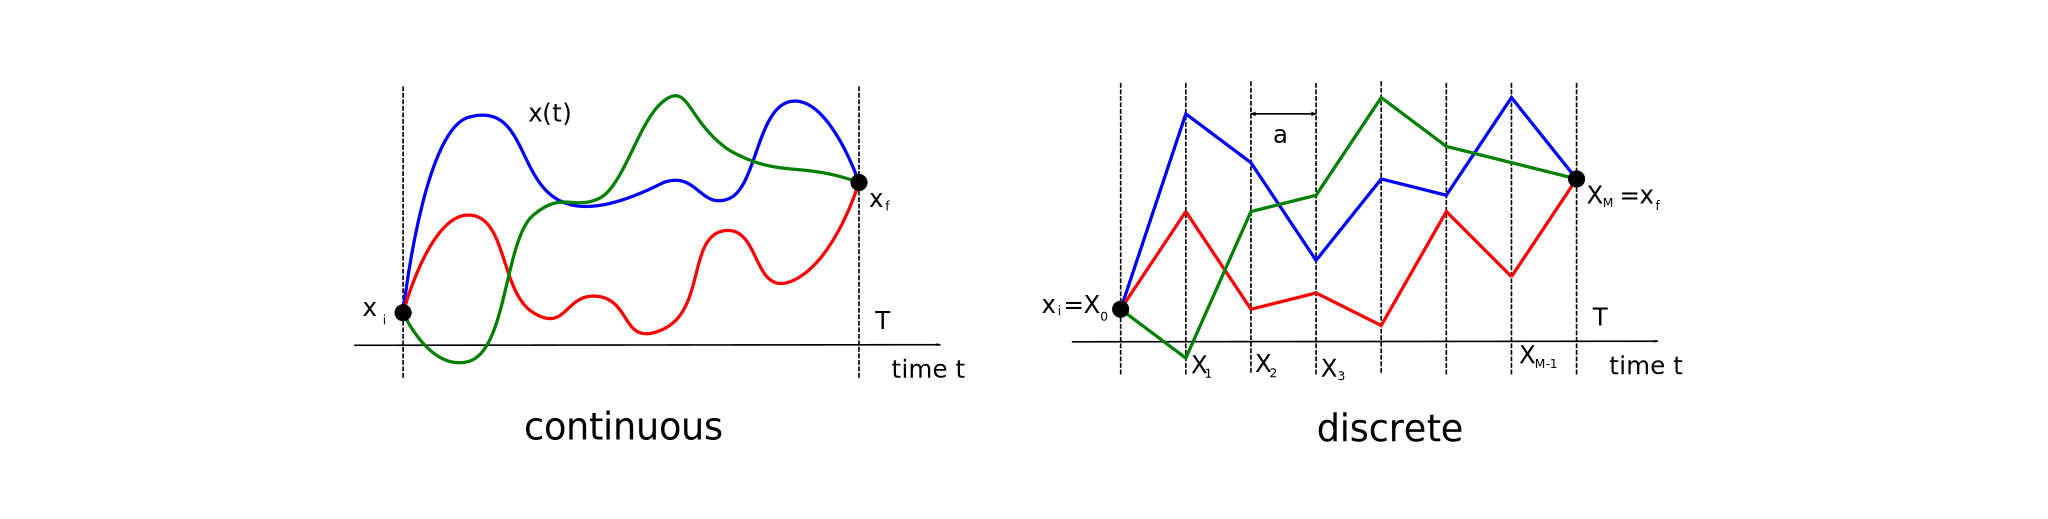
\includegraphics[width=0.5\linewidth]{path_integral.pdf}
\caption{Path integral representation of transition probability $P(b,a)$ in Eq. (\ref{eqn:full_path_integral})}
\label{fig:path_integral}
\end{center}
\end{figure}
%%%%%%%%%%%%%%%%%%%%%%%%%%%%%%%%%%%%%%%%%%%%%%%%%%%%%%%%%%%%%%%%%%%%%%%%
\subsection{Grid hierarchy}
%%%%%%%%%%%%%%%%%%%%%%%%%%%%%%%%%%%%%%%%%%%%%%%%%%%%%%%%%%%%%%%%%%%%%%%%
Introduce a hierarchy of levels $\ell=0,\dots,L$ with $n_\ell=2^\ell$, $h_\ell=T/n_\ell = 2^{-\ell}T$, such that $n=n_L$, i.e. $L$ is the finest level on which we ultimately want to evaluate the path integral. Defining $x^{(\ell)}_k=h_\ell k=T2^{-\ell}k$ we write for the path integral on a particular level $\ell$
\begin{equation}
P^{(\ell)}(b,a) := 
\int\dots\int
P_{h_\ell}(b,x^{(\ell)}_{n_\ell-1})P_{h_\ell}(x^{(\ell)}_{n_\ell-1},x^{(\ell)}_{n_\ell-2})\cdot\dots\cdot
P_{h_\ell}(x^{(\ell)}_2,x^{(\ell)}_1)P_{h_\ell}(x^{(\ell)}_1,a)\;dx^{(\ell)}_1\;dx^{(\ell)}_2\dots dx^{(\ell)}_{n_\ell-1}\label{eqn:level_integral}
\end{equation}
and we want to calculate $P^{(L)}(b,a)$. This is exactly the term under the limit in Eq. (\ref{eqn:full_path_integral}) since $h_L=h$ and $n_L=n$. Note also that $x^{(\ell)}_{2k}=x^{(\ell-1)}_k$, i.e. the even points on a particular level are the points on the next coarser level.
%%%%%%%%%%%%%%%%%%%%%%%%%%%%%%%%%%%%%%%%%%%%%%%%%%%%%%%%%%%%%%%%%%%%%%%%
\subsection{Recursive calculation of $\boldsymbol{P^{(\ell)}(b,a)}$}
%%%%%%%%%%%%%%%%%%%%%%%%%%%%%%%%%%%%%%%%%%%%%%%%%%%%%%%%%%%%%%%%%%%%%%%%
We now show how an estimator for $P^{(\ell)}(b,a)$ can be calculated if $P^{(\ell-1)}(b,a)$ is known.
For this introduce
\begin{equation}
Q^{(\ell-1)}(y_{n_{\ell-1}-1},\dots,y_2,y_1) := \frac{
P_{h_{\ell-1}}(b,y_{n_{\ell-1}-1})\cdot\dots\cdot
P_{h_{\ell-1}}(y_2,y_1)P_{h_{\ell-1}}(y_1,a)
}{P^{(\ell-1)}(b,a)}.\label{eqn:Qc}
\end{equation}
\begin{figure}
\begin{center}
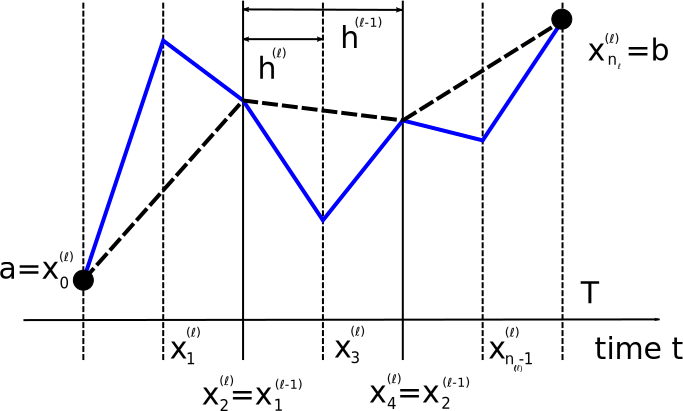
\includegraphics[width=0.5\linewidth]{grid_hierarchy.pdf}
\caption{Paths on different levels: coarse (solid blue) and fine (dashed black).}
\label{fig:grid_hierarchy}
\end{center}
\end{figure}
This is a probability density for the point $(y_1,y_2,\dots,y_{n_{\ell-1}-1})\in\mathbb{R}^{n_{\ell-1}-1}$ since by construction
\begin{equation}
\int\dots\int Q^{(\ell-1)}(y_{n_{\ell-1}-1},\dots,y_2,y_1)\;dy_1\;dy_2\dots dy_{n_{\ell-1}-1} = 1.
\end{equation}
Also, since we know the normalisation $P^{(\ell-1)}(b,a)$, we can evaluate $Q^{(\ell-1)}$ for a given point $(y_1,y_2,\dots,y_{n_{\ell-1}-1})$.

Further define
\begin{equation}
q^{(\ell)}(z;z_+,z_-) := \frac{P_{h_\ell}(z_+,z)P_{h_\ell}(z,z_-)}{\tilde{P}_{2h_\ell}(z_+,z_-)}\qquad\text{with $\tilde{P}_{2h}(z_+,z_-)=\int P_{h}(z_+,z)P_{h}(z,z_-)\;dz$}.\label{eqn:tildeP}
\end{equation}
This is the probability (density) of finding the particle at position $x=z$ at time $t=0$ given that it was at $x=z_-$ at time $t=-h$ and is at time $x=z_+$ at time $t=+h$. $\tilde{P}$ is a function of three variables $(h,z_-,z_+)$. Let's assume that we can somehow calculate this function, possibly numerically to arbitrary precision (in Section \ref{sec:HO} it is calculated explicitly for a harmonic oscillator, $V(x)=\frac{1}{2}\omega^2x^2$). Obviously, per construction
\begin{equation}
\int q^{(\ell)}(z;z_+,z_-)\;dz=1\qquad\text{for any $z_+$, $z_-$}.
\end{equation}
To calculate a Monte Carlo estimator for the integral $P^{(\ell)}(b,a)$ in Eq. (\ref{eqn:level_integral}) we use importance sampling. For this, we generate $M_\ell$ sample paths $(x_1^{(\ell),i},x_2^{(\ell),i},\dots,x_{n_\ell-1}^{(\ell),i})$, $i=1,\dots,M_\ell$ which are distributed according to a known probability density. This is shown in Algorithm \ref{alg:recursive}.
\begin{algorithm}
\begin{algorithmic}[1]
\STATE{Choose $M_\ell$ sets of even points $(x_2^{(\ell),i},x_4^{(\ell),i},\dots,x_{2n_\ell-2}^{(\ell),i})$ distributed according to $Q_c^{(\ell-1)}$, $i=1,\dots,M_\ell$ given in Eq. (\ref{eqn:Qc}). Each set of points can be interpreted as a coarse path, see Fig. \ref{fig:grid_hierarchy}. This can be done efficiently with Hybrid MC. It is very similar to generating states for a spin system or the Ising model.}
\STATE{For each sample $i$, choose the odd points $(x_1^{(\ell),i},x_3^{(\ell),i},\dots,x_{2n_\ell-1}^{(\ell),i})$ such that $x_{2k-1}^{(\ell),i}$ is distributed according to $q^{(\ell)}(\cdot;x_{2k}^{(\ell),i},x_{2k-2}^{(\ell),i})$. This can be done by running a few MCMC iterations to sample from $q^{(\ell)}(\cdot;x_{2k}^{(\ell),i},x_{2k-2}^{(\ell),i})$ for all odd points in parallel.}
\STATE{Given those full sample paths $(x_1^{(\ell),i},x_2^{(\ell),i},\dots,x_{n_\ell-1}^{(\ell),i})$, calculate the Monte Carlo estimator for $P^{(\ell)}(b,a)$ as
\begin{equation}
\hat{P}^{(\ell)}(b,a) = \frac{1}{M_\ell}\sum_{i=1}^{M_\ell}
\frac{
P_{h_\ell}(b,x^{(\ell),i}_{n_\ell-1})P_{h_\ell}(x^{(\ell),i}_{n_\ell-1},x^{(\ell),i}_{n_\ell-2})\cdot\dots\cdot
P_{h_\ell}(x^{(\ell),i}_2,x^{(\ell),i}_1)P_{h_\ell}(x^{(\ell),i}_1,a)
}{Q_c^{(\ell-1)}(x_{n_\ell-2}^{(\ell),i},\dots,x_{4}^{(\ell),i},x_{2}^{(\ell),i})Q_f^{(\ell)}(x_{n_\ell-1}^{(\ell),i},x_{n_\ell-2}^{(\ell),i},\dots,x_{2}^{(\ell),i},x_{1}^{(\ell),i})
}\label{eqn:MCMCestimator}
\end{equation}
where
\begin{equation}
Q^{(\ell)}_f(y_{n_{\ell}-1},y_{n_{\ell}-2},\dots,y_2,y_1):=
q^{(\ell)}(y_{n_\ell-1};b,y_{n_\ell-2})
q^{(\ell)}(y_{n_\ell-3};y_{n_\ell-2},y_{n_\ell-4})\cdot
\dots
\cdot
q^{(\ell)}(y_1;y_2,a).
\end{equation}
}
\end{algorithmic}
\caption{Recursive calculation of MCMC estimator $P^{(\ell)}(b,a)$ given $P^{(\ell-1)}(b,a)$.}
\label{alg:recursive}
\end{algorithm}
For this importance sampling to be successful, the distribution of the samples $(x_1^{(\ell),i},x_2^{(\ell),i},\dots,x_{n_\ell-1}^{(\ell),i})$ has to be approximately proportional to the function we want to integrate, i.e. the integrand in Eq. (\ref{eqn:level_integral}).
This is the case for $h_\ell\rightarrow 0$ since
\begin{equation}
\begin{aligned}
Q_c^{(\ell-1)}(y_{n_\ell-2},\dots,y_2)Q_f^{(\ell)}(y_{n_\ell-1},y_{n_\ell-2},\dots,y_2,y_1)
&=\frac{P_{2h_\ell}(b,y_{n_\ell-2})P_{2h_\ell}(y_{n_\ell-2},y_{n_\ell-4})\cdot\dots\cdot P_{2h_\ell}(y_2,a)}{P^{(\ell-1)}(b,a)}\times\\
&\quad\times
\frac{P_{h_\ell}(b,y_{n_\ell-1})P_{h_\ell}(y_{n_\ell-1},y_{n_\ell-2})\cdot\dots\cdot P_{h_\ell}(y_1,a)}{\tilde{P}_{2h_\ell}(b,y_{n_\ell-2})\cdot\dots\cdot\tilde{P}_{2h_\ell}(y_4,y_2)\tilde{P}_{2h_\ell}(y_2,a)}
\end{aligned}
\end{equation}
For $h_\ell\rightarrow 0$ we have that
\begin{equation}
\tilde{P}_{2h_\ell}(x_{2k},x_{2k-2})\approx P_{2h_\ell}(x_{2k},x_{2k-2})
\label{eqn:P_approx}
\end{equation}
and therefore
\begin{equation}
Q_c^{(\ell-1)}(y_{n_\ell-2,y_{n_\ell-2},\dots,y_2}Q_f^{(\ell)}(y_{n_\ell-1},\dots,y_2,y_1)
\approx 
\frac{P_{h_\ell}(b,y_{n_\ell-1})P_{h_\ell}(y_{n_\ell-1},y_{n_\ell-2})\cdot\dots\cdot P_{h_\ell}(y_1,a)}{P^{(\ell-1)}(b,a)}
\label{eqn:distribution_equivalence}
\end{equation}
as required.
%%%%%%%%%%%%%%%%%%%%%%%%%%%%%%%%%%%%%%%%%%%%%%%%%%%%%%%%%%%%%%%%%%%%%%%%
\subsection{Multilevel algorithm}
%%%%%%%%%%%%%%%%%%%%%%%%%%%%%%%%%%%%%%%%%%%%%%%%%%%%%%%%%%%%%%%%%%%%%%%%
Hence the multilevel calculation of an Monte Carlo estimator $\hat{P}^{(L)}(b,a)$ works as shown in Algorithm \ref{alg:multilevel}.
\begin{algorithm}
\begin{algorithmic}[1]
\STATE{Choose the number of samples $M_\ell$ for $\ell=1,\dots,L$.}
\STATE{Set $\hat{P}^{(0)}(b,a) = P_T(b,a)$ with $P_T$ defined in Eq. (\ref{eqn:transition_probability}).}
\FOR{$\ell=1$ \TO $L$}
\STATE{Given $\hat{P}^{(\ell-1)}(b,a)$ on the previous level, calculate an Monte Carlo estimator $\hat{P}^{(\ell)}(b,a)$ with $M_\ell$ samples according to Algorithm \ref{alg:recursive}.}
\ENDFOR
\end{algorithmic}
\caption{Multilevel algorithm}\label{alg:multilevel}
\end{algorithm}
For the finer levels we need less samples, since the the sample distribution is good (see Eq. (\ref{eqn:distribution_equivalence})). For the coarser levels we need more samples, but they are cheaper. We therefore expect heuristically that $M_1\gg M_2\gg\dots\gg M_L$.
%%%%%%%%%%%%%%%%%%%%%%%%%%%%%%%%%%%%%%%%%%%%%%%%%%%%%%%%%%%%%%%%%%%%%%%%
\section{Harmonic oscillator}\label{sec:HO}
%%%%%%%%%%%%%%%%%%%%%%%%%%%%%%%%%%%%%%%%%%%%%%%%%%%%%%%%%%%%%%%%%%%%%%%%
Consider $V(x)=\frac{1}{2}\omega^2x^2$. In this case we can calculate $\tilde{P}_{2h}(z_+,z_-)$ defined in Eq. (\ref{eqn:tildeP}) with forward Euler timestepping exactly as
\begin{equation}
\begin{aligned}
\tilde{P}_{2h}(z_+,z_) &=
\int P_h(z_+,z)P_h(z,z_-)\;dz = 
\frac{1}{2\pi\sigma^2 h}\int
\exp\left[-\frac{(z_+-z+hV'(z))^2+(z-z_-+hV'(z_-))^2}{2\sigma^2h}
\right]\;dz\\
&=\frac{1}{2\pi\sigma^2 h}\int
\exp\left[-\frac{((1-\omega^2h)z-z_+)^2+(z-(1-\omega^2h)z_-)^2}{2\sigma^2h}\right]\;dz
\end{aligned}
\end{equation}
To evaluate this Gaussian integral, use
\begin{equation}
\begin{aligned}
((1-\omega^2h)z-z_+)^2 + (z-(1-\omega^2h)z_-)^2 
&= (1-\omega^2h)^2 z^2 - 2(1-\omega^2h)z_+ z + z_+^2
+ z^2 -2(1-\omega^2h)z_-z+(1-\omega^2h)^2z_-^2\\
&= \left[(1-\omega^2h)^2+1\right]z^2-2\left[(1-\omega^2h)(z_++z_-)\right]+z_+^2+(1-\omega^2h)^2z_-^2\\
&= \left[(1-\omega^2h)^2+1\right]\left[
z^2 - 2\frac{(1-\omega^2h)(z_++z_-)}{(1-\omega^2h)^2+1} + \frac{(1-\omega^2h)^2(z_++z_-)^2}{((1-\omega^2h)^2+1)^2}
\right]\\
&\qquad-\;\;\frac{(1-\omega^2h)^2(z_++z_-)^2}{(1-\omega^2h)^2+1} + z_+^2 + (1-\omega^2h)^2z_-^2\\
&= \left[(1-\omega^2h)^2+1\right](z-g_{\omega^2h}(z_+,z_-))^2 + \frac{1}{2}r_{\omega^2h}(z_+,z_-)
\end{aligned}
\end{equation}
where $g_s(z_+,z_-)$ is some (irrelevant) function of $z_+$ and $z_-$ and
\begin{equation}
r_s(z_+,z_-) = 2z_+^2+2(1-s)^2z_-^2 - \frac{2(1-s)^2(z_++z_-)^2}{(1-s)^2+1} = (z_+-z_-)^2+\mathcal{O}(s).
\end{equation}
Therefore
\begin{equation}
\begin{aligned}
\tilde{P}_{2h}(z_+,z_-) &= \frac{1}{2\pi\sigma^2 h}
\exp\left[
-\frac{r_{\omega^2h}(z_+,z_-)}{4\sigma^2h}
\right]
\int 
\exp\left[
-\frac{(1-\omega^2h)^2+1}{2\sigma^2h}(z-g_{\omega^2h}(z_+,z_-))^2
\right]\;dz
\end{aligned}
\end{equation}
The integral is readily evaluated to
\begin{equation}
\begin{aligned}
\int 
\exp\left[
-\frac{(1-\omega^2h)^2+1}{2\sigma^2h}(z-g_{\omega^2h}(z_+,z_-))^2
\right]\;dz &= 
\int 
\exp\left[
-\frac{(1-\omega^2h)^2+1}{2\sigma^2h}z^2
\right]\;dz\\
&= \sqrt{\frac{2\pi\sigma^2 h}{(1-\omega^2h)^2+1}} = \sqrt{\pi\sigma^2h}+\mathcal{O}(\omega^2h)
\end{aligned}
\end{equation}
Taking everything together we have
\begin{equation}
\begin{aligned}
\tilde{P}_{2h}(z_+,z_-) &= \frac{1}{\sqrt{4\pi\sigma^2 h}}\sqrt{\frac{2}{(1-\omega^2h)^2+1}}
\exp\left[
-\frac{r_{\omega^2h}(z_+,z_-)}{4\sigma^2h}
\right] = \underbrace{\frac{1}{\sqrt{4\pi\sigma^2h}}\exp\left[
-\frac{(z_+-z_-)^2}{4\sigma^2h}\right]}_{P_{2h}(z_+,z_-)}+\mathcal{O}(\omega^2h)
\end{aligned}
\end{equation}
which confirms Eq. (\ref{eqn:P_approx}) in this case since $\tilde{P}_{2h}(z_+,z_-)=P_{2h}(z_+,z_-)+\mathcal{O}(\omega^2h)$. In fact, for $\omega=0$ (no potential, $V(x)=0$) we have $\tilde{P}_{2h}(z_+,z_-)=P_{2h}(z_+,z_-)$ for all $h$. This is expected, since in this case the transition probability for any $T$ is exactly $P(b,a)=\frac{1}{\sqrt{2\pi\sigma^2T}}\exp\left[-\frac{(b-a)^2}{2\sigma^2T}\right]$. In this case the algorithm becomes trivial since the ratio in Eq. (\ref{eqn:MCMCestimator}) is 1 and $\hat{P}^{(\ell)}(b,a)=P^{(\ell)}(b,a)=P(b,a)$ for all $\ell$.
\end{document}
